\section{Exploratory Data Analysis}
\label{sec:eda}

Detailed EDA was restricted to the official training split. The test file was inspected only for schema and integrity, preventing test-label observations from influencing feature or model choices. The analysis covers data quality, class balance, tweet length and structure, and frequent words and bigrams.

\subsection{Data Quality}

Neither split contains missing tweet text, missing labels, empty text, or exact duplicate rows. Normalized text comparison identified 28 training rows belonging to duplicate-text groups, with no conflicting labels. One normalized tweet appeared in both training and test. Before model development, the test-overlapping training row was removed and repeated training texts were reduced to one row per normalized text. This produced 41,141 clean training rows.

\begin{table}[H]
\centering
\begin{tabular}{|l|r|r|}
\hline
Quality check & Training & Test \\
\hline
Rows & 41,157 & 3,798 \\
\hline
Missing tweet text & 0 & 0 \\
\hline
Missing sentiment & 0 & 0 \\
\hline
Empty tweet text & 0 & 0 \\
\hline
Exact duplicate rows & 0 & 0 \\
\hline
Rows in duplicate-text groups & 28 & 0 \\
\hline
Duplicate groups with conflicting labels & 0 & 0 \\
\hline
Unique train/test text overlap & \multicolumn{2}{|c|}{1} \\
\hline
\end{tabular}
\caption{Raw data-quality audit.}
\label{tab:data-quality}
\end{table}

\subsection{Class Distribution}

The largest class is Positive with 11,422 tweets (27.75\%), while Extremely Negative is the smallest with 5,481 tweets (13.32\%). The imbalance is moderate but meaningful. This observation motivates macro-averaged F1 as the primary model-selection metric because it gives equal importance to every class.

\begin{figure}[H]
\centering
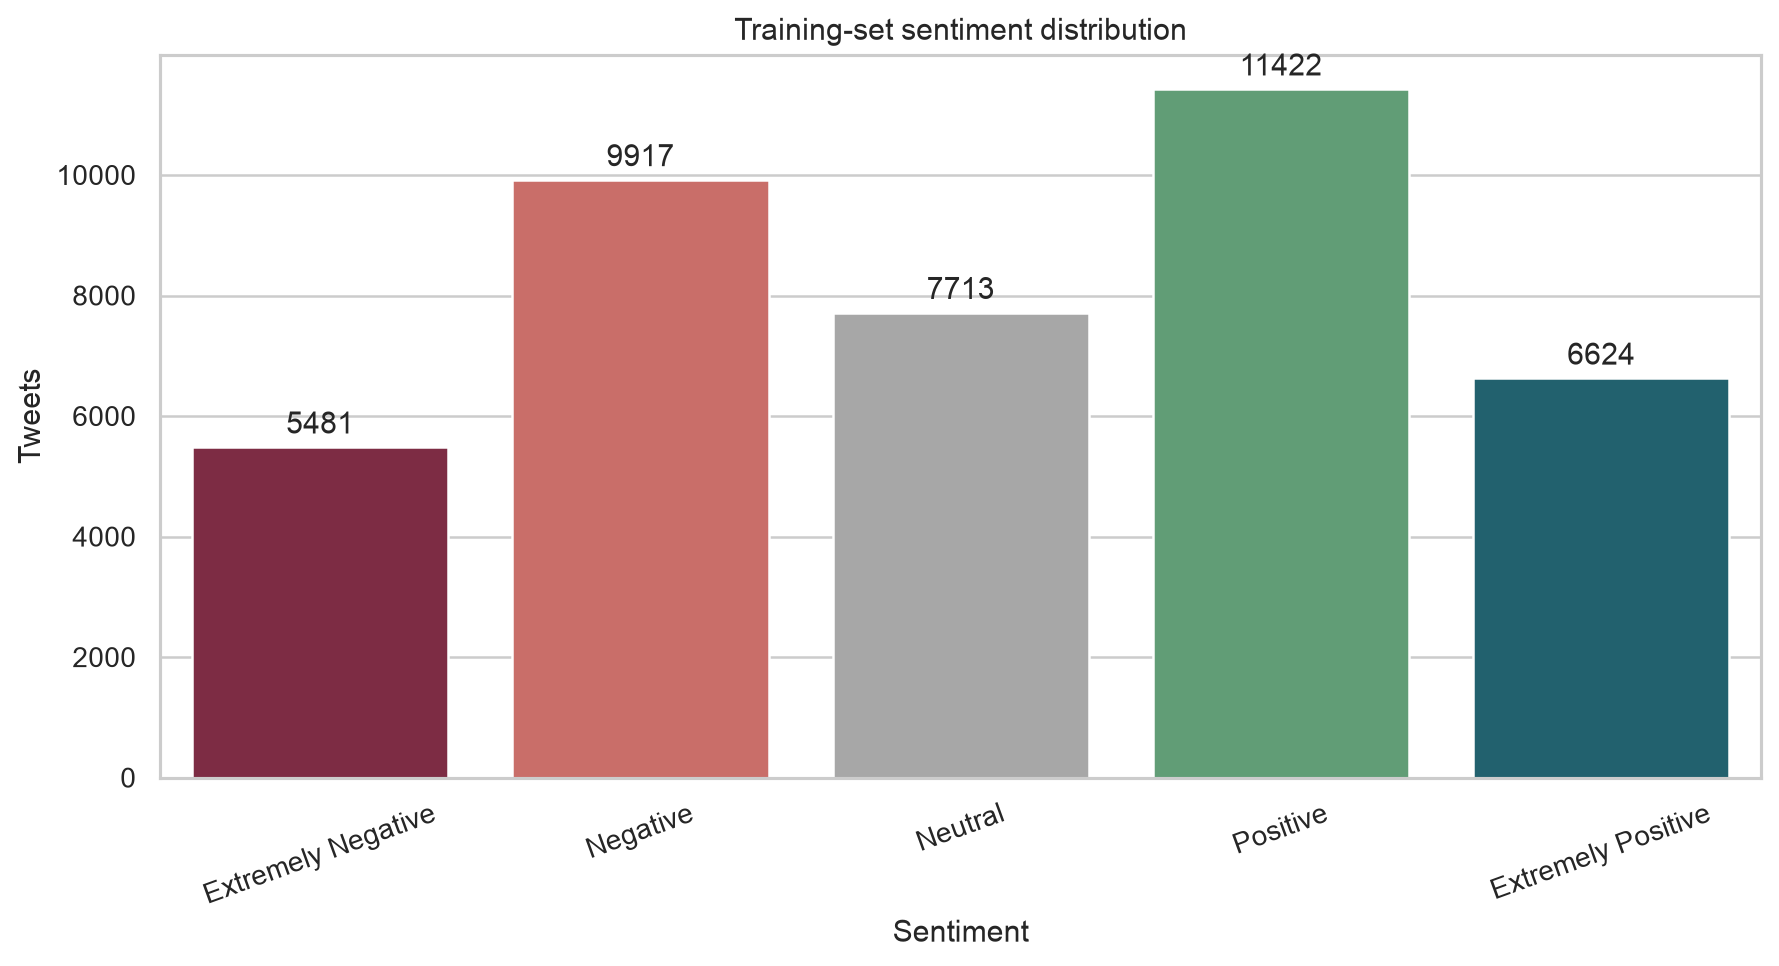
\includegraphics[width=0.94\textwidth]{../outputs/graphics/eda/class_distribution.png}
\caption{Sentiment distribution in the official training set.}
\label{fig:class-distribution}
\end{figure}

\begin{table}[H]
\centering
\begin{tabular}{|l|r|r|}
\hline
Sentiment & Count & Percentage \\
\hline
Extremely Negative & 5,481 & 13.32\% \\
\hline
Negative & 9,917 & 24.10\% \\
\hline
Neutral & 7,713 & 18.74\% \\
\hline
Positive & 11,422 & 27.75\% \\
\hline
Extremely Positive & 6,624 & 16.09\% \\
\hline
\end{tabular}
\caption{Training-set class distribution.}
\label{tab:class-distribution}
\end{table}

\subsection{Tweet Length and Structure}

Across all 41,157 training tweets, the mean length is 32.93 words (standard deviation 11.80) and the median is 34 words. The middle 50\% spans 24--42 words, and the observed range is 1--66 words. Character counts have a mean of 204.20, a median of 215, and an observed range of 11--355. Table~\ref{tab:length-summary} makes the word-count statistics explicit, while Figure~\ref{fig:text-length} shows the complete word- and character-length distributions.

\begin{table}[H]
\centering
\small
\setlength{\tabcolsep}{4pt}
\begin{tabular}{|l|r|r|r|r|r|r|r|r|}
\hline
Measure & Mean & SD & Min & Q1 & Median & Q3 & P95 & Max \\
\hline
Words & 32.93 & 11.80 & 1 & 24 & 34 & 42 & 50 & 66 \\
\hline
Characters & 204.20 & 68.66 & 11 & 151 & 215 & 259 & 300 & 355 \\
\hline
\end{tabular}
\caption{Training-set text-length summary. Q1 and Q3 are the 25th and 75th percentiles.}
\label{tab:length-summary}
\end{table}

Neutral tweets are shorter, with a median of 24 words, compared with medians of 34 words for Negative and Positive and 38 words for both extreme classes. This suggests that strongly expressed sentiment often uses more text, while neutral statements are more concise. Approximately 48.16\% of training tweets contain a URL, 23.62\% contain a mention, and 57.63\% contain a hashtag. These elements are common enough to require explicit handling rather than accidental deletion.

\begin{figure}[H]
\centering
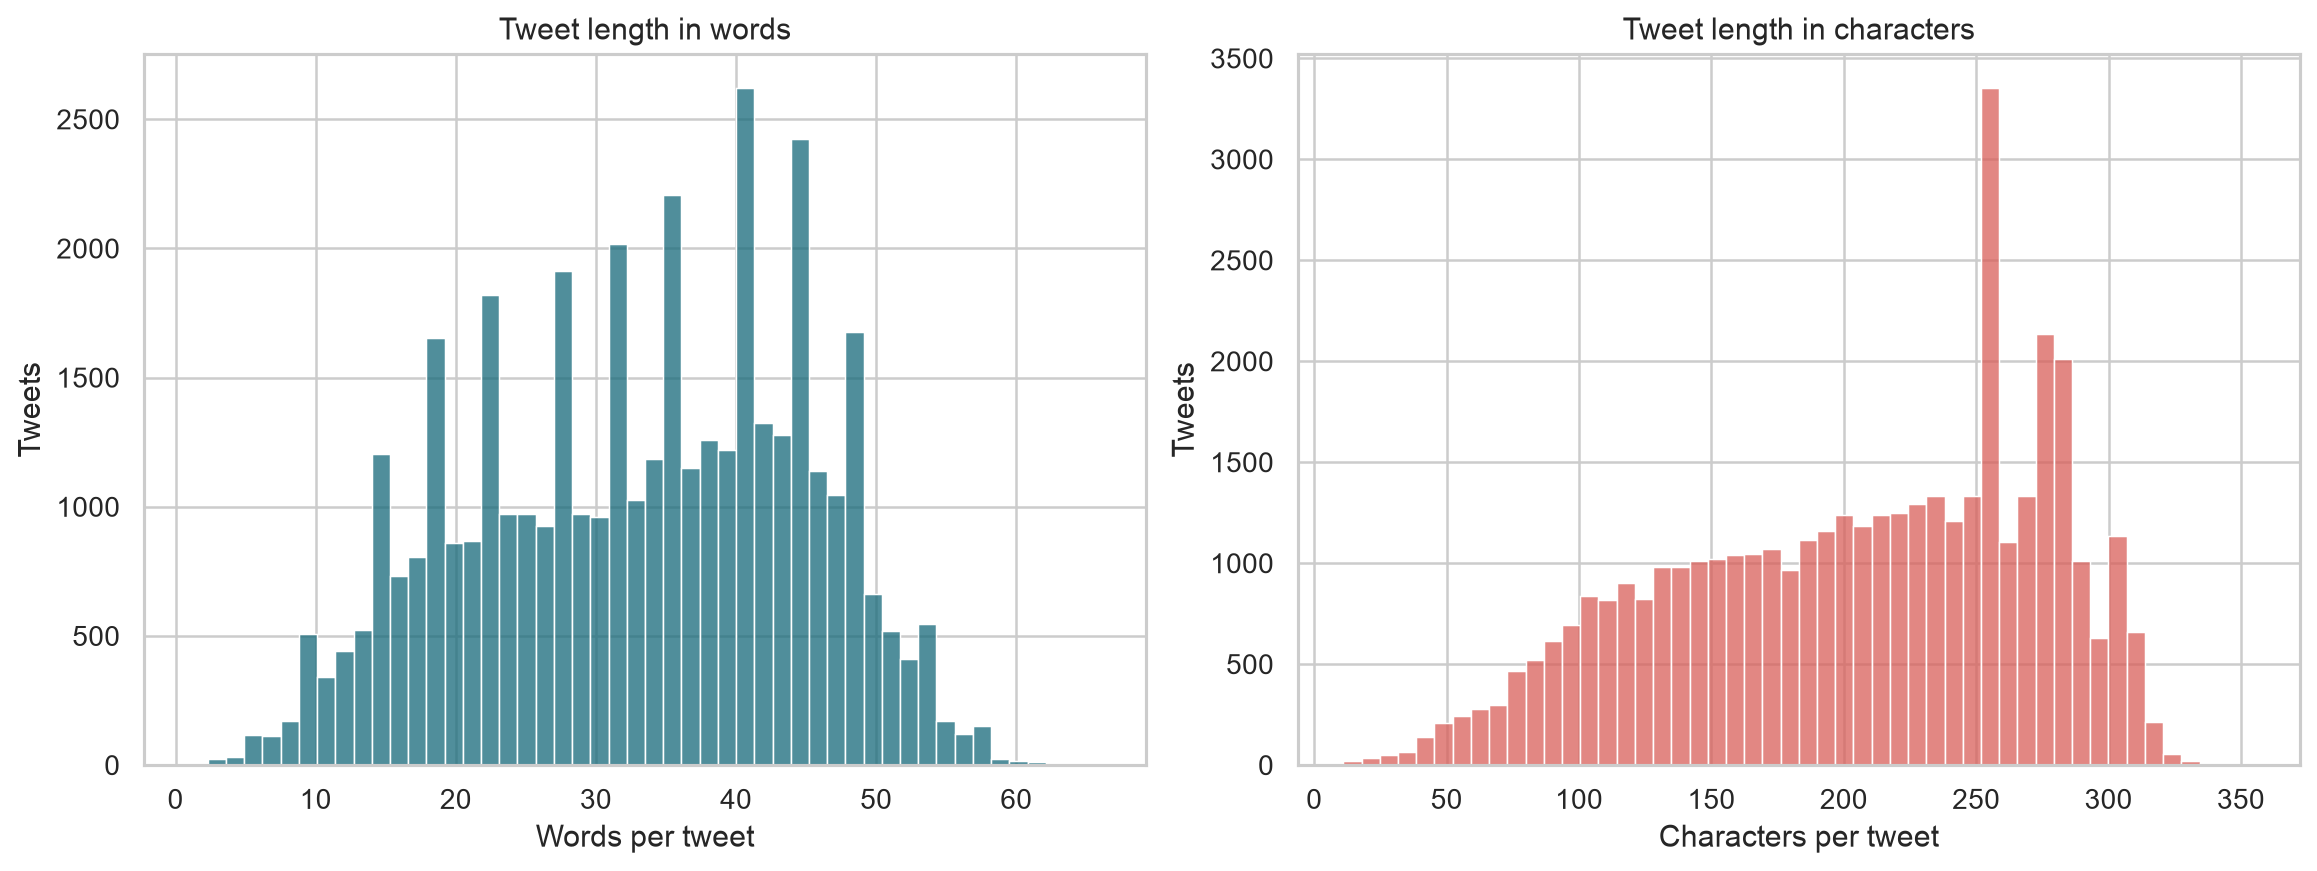
\includegraphics[width=\textwidth]{../outputs/graphics/eda/text_length_distributions.png}
\caption{Training tweet length measured in words and characters.}
\label{fig:text-length}
\end{figure}

\begin{figure}[H]
\centering
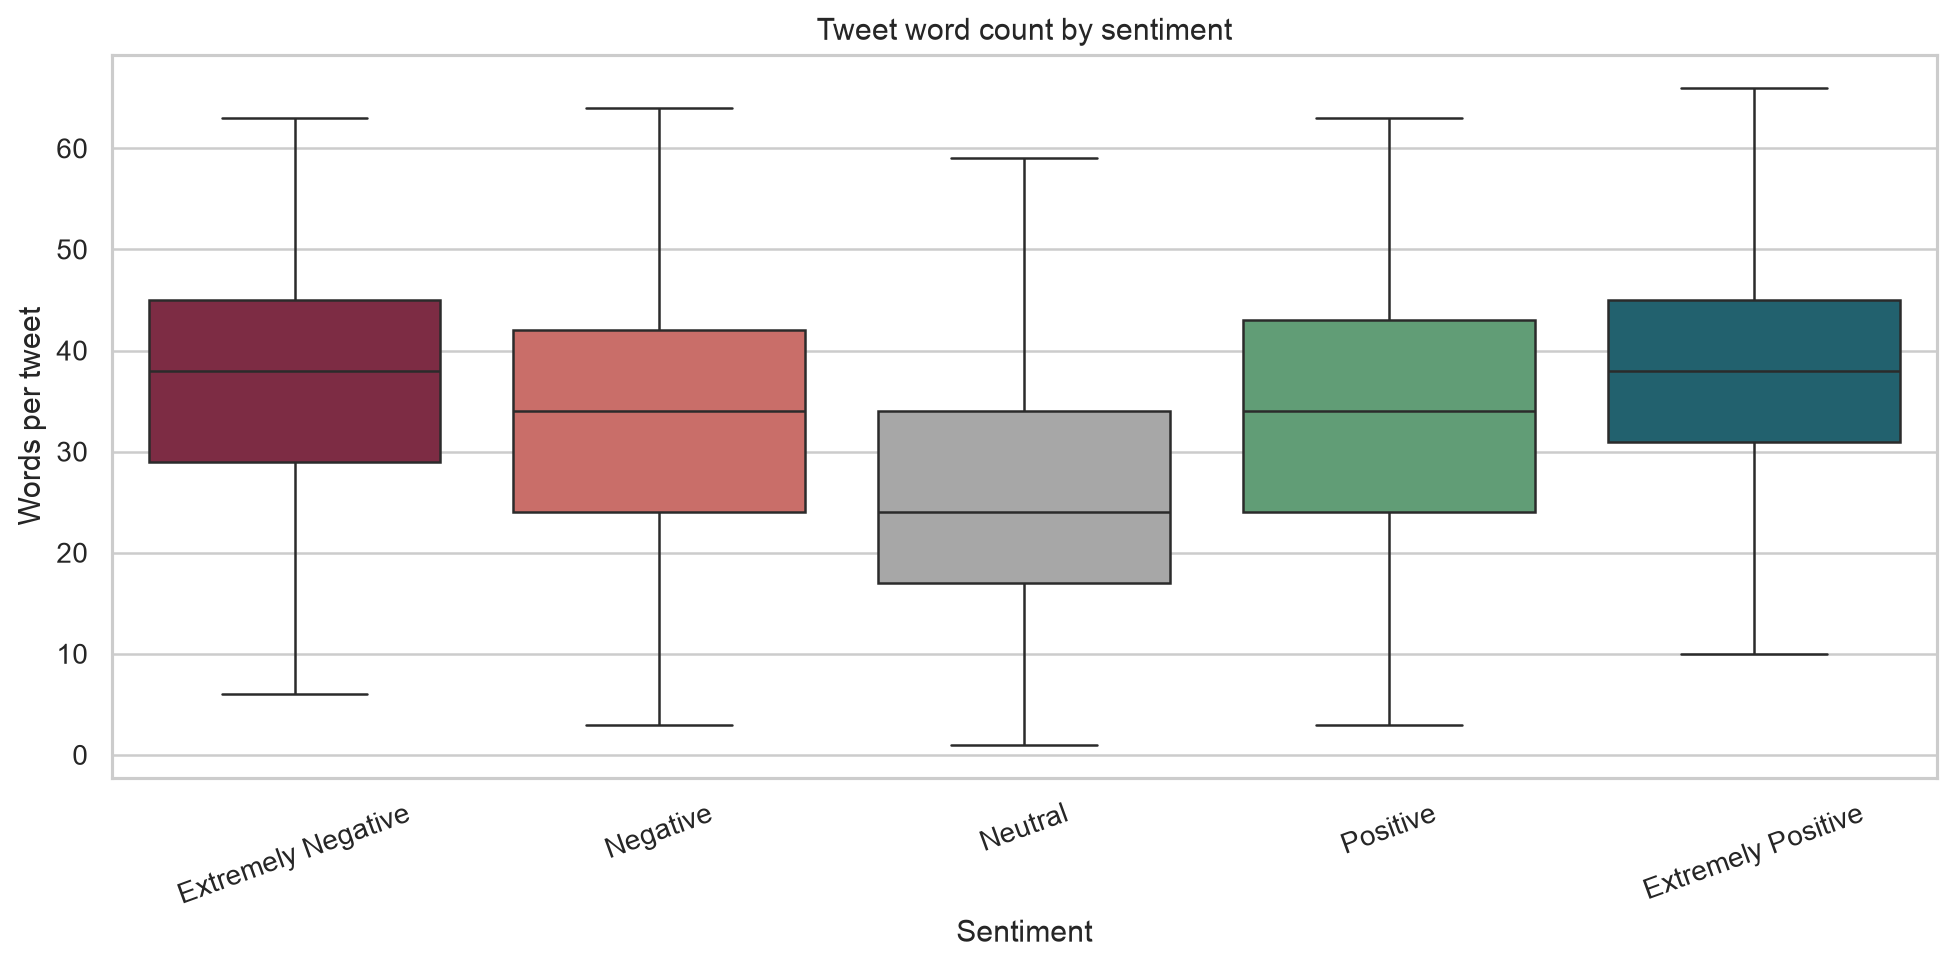
\includegraphics[width=\textwidth]{../outputs/graphics/eda/word_count_by_sentiment.png}
\caption{Word-count distribution by sentiment class; outliers are hidden for readability.}
\label{fig:word-count-sentiment}
\end{figure}

\subsection{Frequent Words and Bigrams}

For descriptive frequency plots only, URLs, mentions, HTML artifacts, and a compact stop-word list were removed. The most frequent words include \textit{covid}, \textit{coronavirus}, \textit{prices}, \textit{food}, \textit{supermarket}, and \textit{grocery}. Frequent bigrams include \textit{grocery store}, \textit{hand sanitizer}, \textit{online shopping}, \textit{toilet paper}, and \textit{panic buying}. The corpus therefore reflects both public-health discussion and consumer-supply concerns. This descriptive cleanup is separate from the modeling preprocessing described in Section~\ref{sec:pipeline}.

The leading unigram counts were \textit{covid} (23,222), \textit{coronavirus} (18,207), \textit{prices} (7,957), \textit{food} (7,178), \textit{supermarket} (7,085), and \textit{store} (6,922). The most frequent bigram was \textit{grocery store} (4,776), followed by \textit{coronavirus covid} (2,431), \textit{covid coronavirus} (1,976), \textit{hand sanitizer} (1,543), and \textit{online shopping} (1,359). These counts provide a numeric counterpart to Figures~\ref{fig:top-unigrams} and~\ref{fig:top-bigrams}.

\begin{figure}[H]
\centering
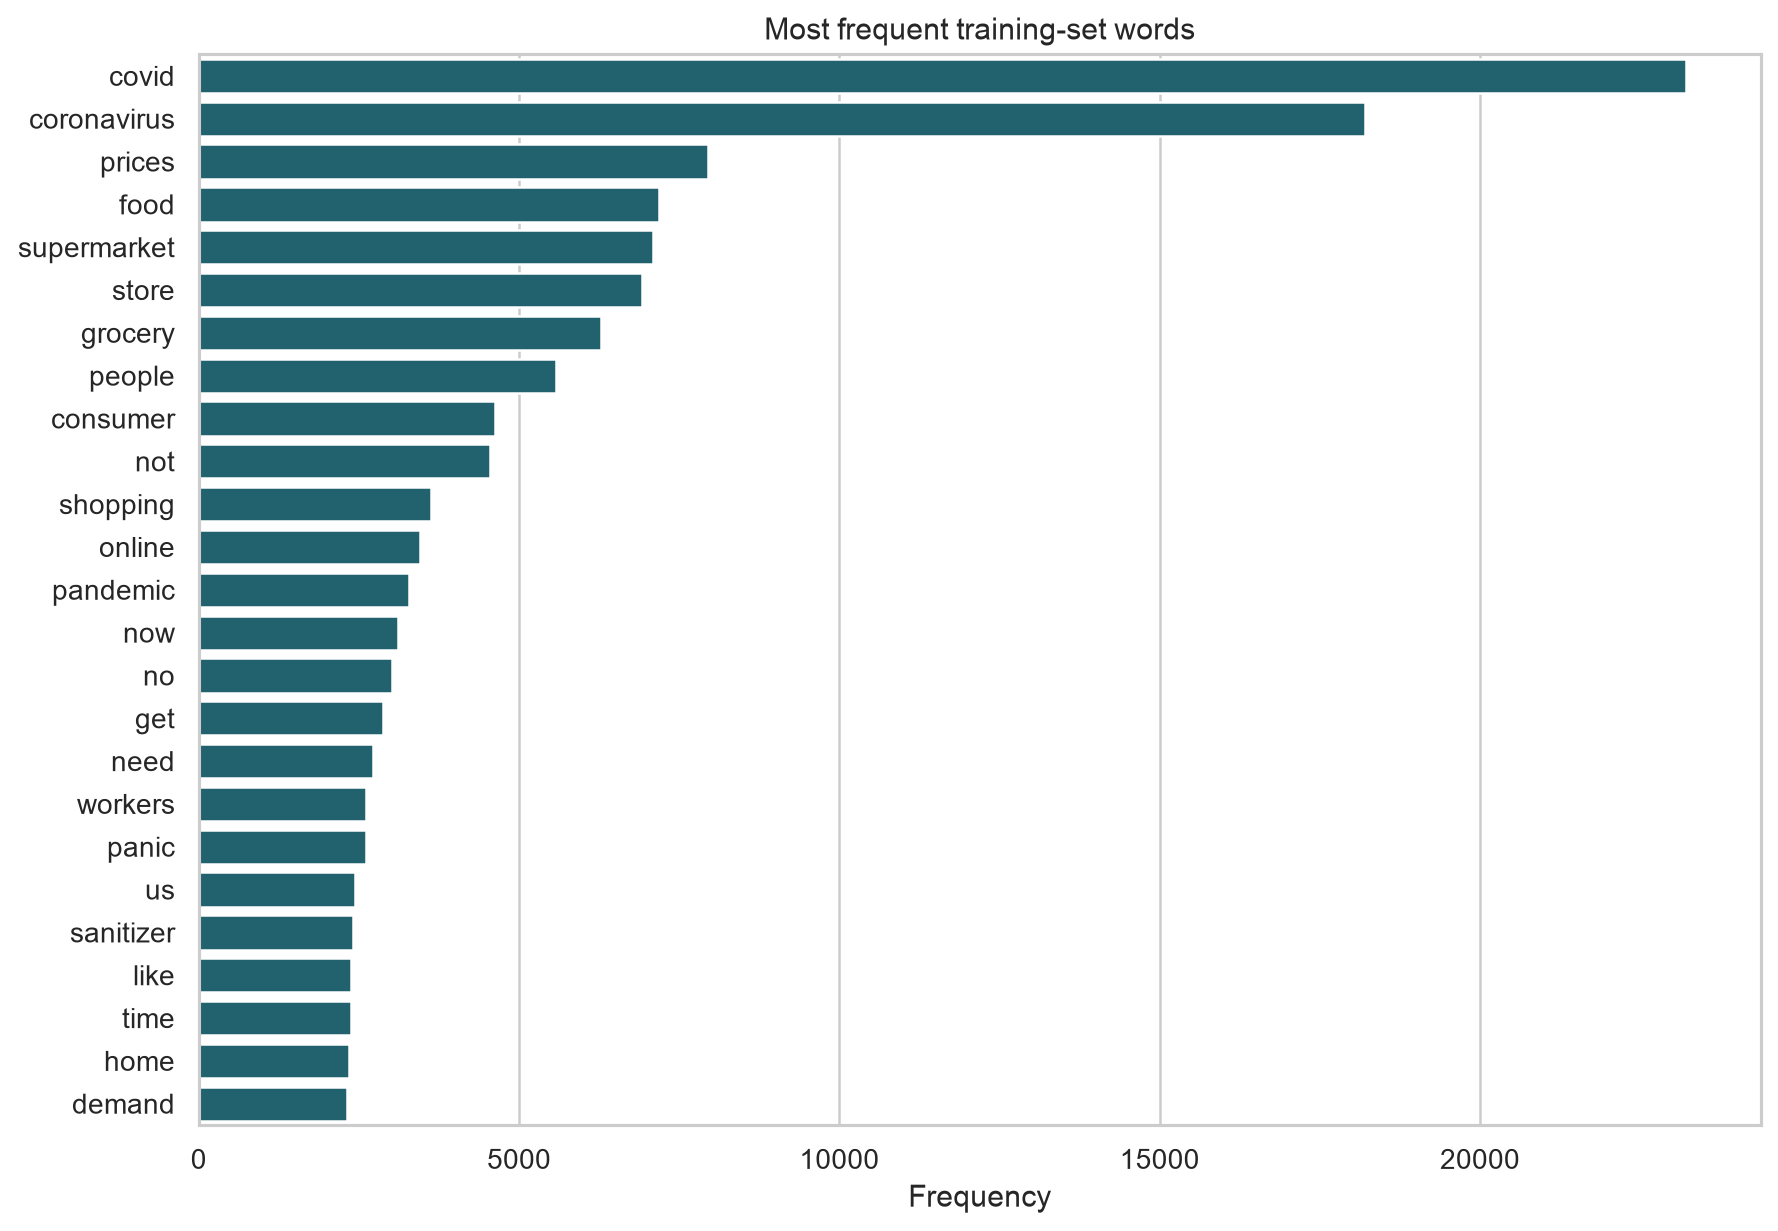
\includegraphics[width=0.88\textwidth]{../outputs/graphics/eda/top_unigrams.png}
\caption{Most frequent words in the training tweets after descriptive cleanup.}
\label{fig:top-unigrams}
\end{figure}

\begin{figure}[H]
\centering
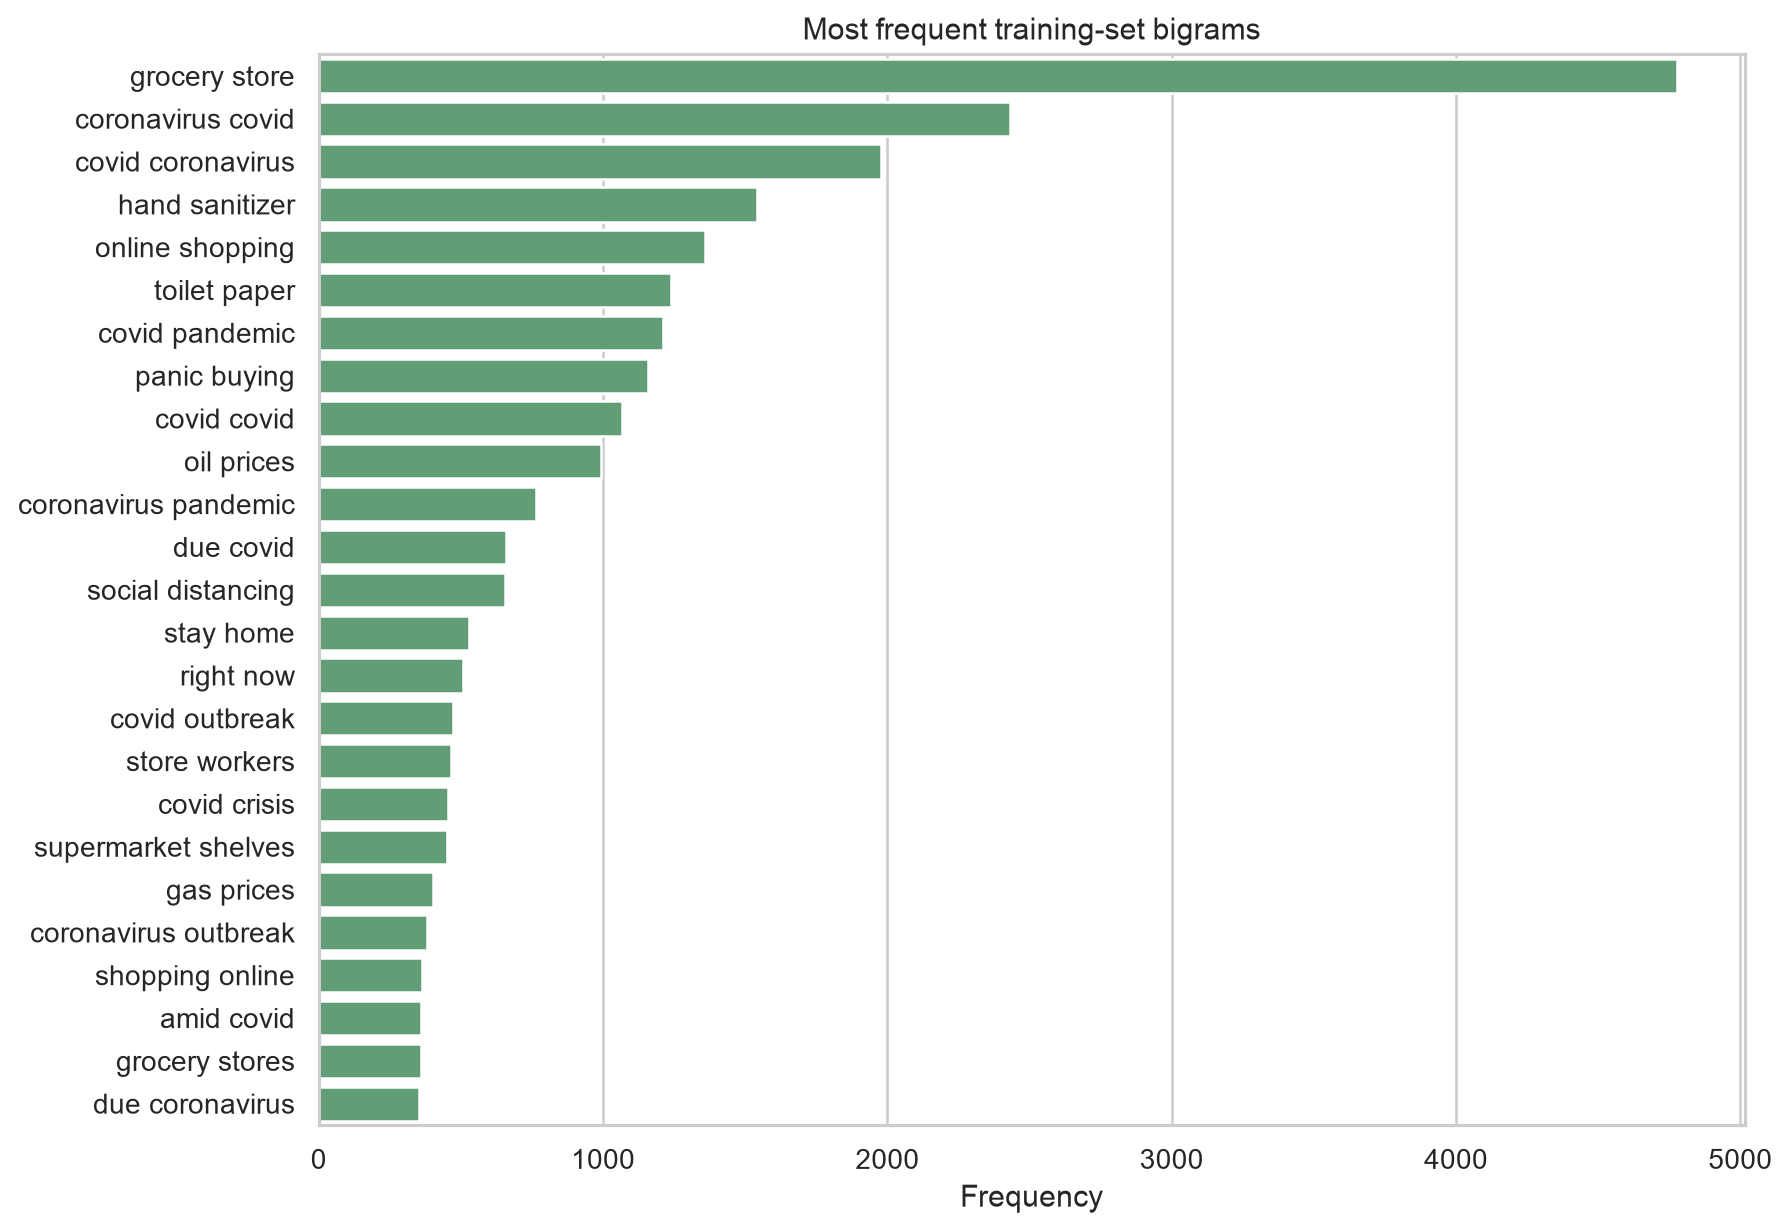
\includegraphics[width=0.88\textwidth]{../outputs/graphics/eda/top_bigrams.png}
\caption{Most frequent bigrams in the training tweets after descriptive cleanup.}
\label{fig:top-bigrams}
\end{figure}

EDA identifies three design requirements for the pipeline: preserve sentiment-bearing negation, handle URLs and mentions explicitly, and use stratified evaluation with a class-balanced metric.
